\documentclass[11pt]{article}

% --- Packages ---
\usepackage[utf8]{inputenc}
\usepackage[T1]{fontenc}
\usepackage{lmodern}
\usepackage[margin=1in]{geometry}
\usepackage{amsmath, amssymb, amsthm, mathtools}
\usepackage{listings}
\usepackage{xcolor}
\usepackage{hyperref}
\usepackage{cleveref}
\usepackage{tikz}

\crefname{theorem}{Theorem}{Theorems}
\Crefname{theorem}{Theorem}{Theorems}
\crefname{lemma}{Lemma}{Lemmas}
\Crefname{lemma}{Lemma}{Lemmas}
\crefname{proposition}{Proposition}{Propositions}
\Crefname{proposition}{Proposition}{Propositions}
\crefname{corollary}{Corollary}{Corollaries}
\Crefname{corollary}{Corollary}{Corollaries}
\crefname{definition}{Definition}{Definitions}
\Crefname{definition}{Definition}{Definitions}
\crefname{example}{Example}{Examples}
\Crefname{example}{Example}{Examples}
\crefname{remark}{Remark}{Remarks}
\Crefname{remark}{Remark}{Remarks}

% --- Theorem environments ---
\theoremstyle{plain}
\newtheorem{theorem}{Theorem}[section]
\newtheorem{lemma}[theorem]{Lemma}
\newtheorem{proposition}[theorem]{Proposition}
\newtheorem{corollary}[theorem]{Corollary}

\theoremstyle{definition}
\newtheorem{definition}[theorem]{Definition}
\newtheorem{example}[theorem]{Example}

\theoremstyle{remark}
\newtheorem{remark}[theorem]{Remark}

% --- Lean listing setup ---
\definecolor{leankeyword}{RGB}{0,0,180}
\definecolor{leancomment}{RGB}{100,100,100}
\definecolor{leanstring}{RGB}{160,0,0}
\definecolor{leanbg}{RGB}{248,248,248}

\lstdefinelanguage{lean}{
  morekeywords={
    theorem,lemma,definition,def,example,axiom,structure,inductive,class,instance,
    variable,variables,namespace,end,open,import,section,universe,universes,
    fun,let,in,if,then,else,match,with,do,return,have,show,by,from,this,
    suffices,calc,Type,Prop,Sort,Pi,forall,exists,
    where,deriving,abbrev,notation,infixl,infixr,prefix,postfix,mutual
  },
  sensitive=true,
  morecomment=[l]{--},
  morecomment=[s]{/-}{-/},
  morestring=[b]",
  literate=
    {α}{{$\alpha$}}1 {β}{{$\beta$}}1 {γ}{{$\gamma$}}1 {δ}{{$\delta$}}1
    {ε}{{$\varepsilon$}}1 {λ}{{$\lambda$}}1 {μ}{{$\mu$}}1 {σ}{{$\sigma$}}1
    {τ}{{$\tau$}}1 {φ}{{$\varphi$}}1 {ψ}{{$\psi$}}1 {ω}{{$\omega$}}1
    {Γ}{{$\Gamma$}}1 {Δ}{{$\Delta$}}1 {Σ}{{$\Sigma$}}1 {Π}{{$\Pi$}}1
    {ℕ}{{$\mathbb{N}$}}1 {ℤ}{{$\mathbb{Z}$}}1 {ℚ}{{$\mathbb{Q}$}}1
    {ℝ}{{$\mathbb{R}$}}1 {ℂ}{{$\mathbb{C}$}}1
    {→ₗ}{{$\to_{\ell}$}}1 {≃ₗ}{{$\simeq_{\ell}$}}1 {ₗ}{{$_{\ell}$}}1
    {→}{{$\to$}}1 {↦}{{$\mapsto$}}1 {⟶}{{$\longrightarrow$}}1
    {∀}{{$\forall$}}1 {∃}{{$\exists$}}1 {¬}{{$\neg$}}1
    {∧}{{$\wedge$}}1 {∨}{{$\vee$}}1 {↔}{{$\leftrightarrow$}}1
    {∣}{{$\mid$}}1
    {≤}{{$\leq$}}1 {≥}{{$\geq$}}1 {≠}{{$\neq$}}1 {≡}{{$\equiv$}}1
    {∈}{{$\in$}}1 {∉}{{$\notin$}}1 {⊆}{{$\subseteq$}}1 {⊂}{{$\subset$}}1
    {⧸}{{$/$}}1
    {∪}{{$\cup$}}1 {∩}{{$\cap$}}1 {∅}{{$\emptyset$}}1
    {⟨}{{$\langle$}}1 {⟩}{{$\rangle$}}1 {·}{{$\cdot$}}1 {∘}{{$\circ$}}1
}

\lstset{
  language=lean,
  basicstyle=\ttfamily\small,
  keywordstyle=\color{leankeyword}\bfseries,
  commentstyle=\color{leancomment}\itshape,
  stringstyle=\color{leanstring},
  backgroundcolor=\color{leanbg},
  frame=single,
  rulecolor=\color{black!20},
  showstringspaces=false,
  breaklines=true,
  breakatwhitespace=true,
  columns=fullflexible,
  keepspaces=true,
  numbers=left,
  numberstyle=\tiny\color{gray},
  numbersep=8pt,
  xleftmargin=2.5em,
  framexleftmargin=2em,
  captionpos=b,
}

% Shorthand for inline Lean code
\newcommand{\lean}[1]{\lstinline[language=lean]|#1|}

% --- Metadata ---
\title{ChainCert: Certified Simplicial Homology Computations in Lean Using Sage}
\author{Lucy Horowitz}
\date{May 16, 2026}

\begin{document}
\maketitle

\begin{abstract}
A short summary of what was formalized, why it matters, and the main results.
\end{abstract}

\section{Introduction}\label{sec:intro}
Interactive theorem provers (ITPs) like Lean are very good at checking proofs but not so good at computing. Computer algebra systems (CAS) like Sage are very good at computing but offer no formal guarantees on their answers. Large parts of modern mathematics already rely on CAS, and with recent rapid strides in autoformalization, more mathematics is formalized every day. There is still a critical gap, however, between ``what the CAS said'' and ``what we've formally proved'' if we want to use CAS results downstream in proofs. 

In theory it is possible to re-implement the necessary algorithms in Lean or prove that the implementation in Sage is correct, but this is difficult. Algorithms may be enormously complicated or rely on space-saving hacks for efficiency that Lean isn't able to take advantage of. Moreover, Lean isn't built for numerical work in the first place.

Another strategy to solve this problem is to let each system do what it is good at at build a concrete bridge between them. Instead of blindly trusting Sage's answer, we can modify what it outputs so that Lean is capable of checking the answer. The output is a \textit{certificate} of computation: a small amount of additional data that is sufficient for the verification of the result. This moves the trust boundary from all of Sage to Lean's typechecker. This general pattern of certificate-based CAS-Lean interaction follows Baanen et al. \cite{baanenCertifyingRingsIntegers2025}.

This project develops the paradigm for the concrete case of integral homology of a finite simplicial complex. Computing the homology groups is simple and well-understood: it takes nothing more than computing the boundary matrices, computing two Smith normal forms, and reading off the invariant factors. If you ask Sage to compute the homology groups of a simplicial complex it will just give you the Betti numbers and torsion coefficients, not any of the intermediate matrices. With just these numbers alone, it is not possible to check whether or not the answer is correct. We instead ask sage for a full certificate, including the Smith normal forms (which have their own certificates) and prove a theorem in Lean that this is sufficient to guarantee correctness of the computation. 

Homology is a useful first target for this kind of certificate-based bridge because the underlying linear algebra is concrete and well-understood, the certificates are small and easy to specify, while the workflow exposes every part of the interface between Sage and Lean, from serialization of ring elements to parsing structured output and constructing \lean{Expr}s.

The rest of the paper is strucutred as follows: \Cref{sec:background} reviews the mathematical backround necessary for computing the homology groups of a simplicial complex using the SNF. It is short and self-contained beyond some basic facts and definitions in algebra and topology. \cref{sec:certificates} introduces the certificates we defined and proves their soundness. \cref{sec:tactics} describes the Lean tactics and commands that work with the certificates. \cref{sec:theorems} collects the main verified ``bridge theorems.'' \cref{sec:examples} works through concrete examples, and \cref{sec:future} describes potential future directions for the project. 


\section{Background}\label{sec:background}
\subsection{Smith Normal Form}
Let $R$ be a principal ideal domain. For the purposes of this project, we will always be dealing with the integers, but the results work more generally. 

\begin{definition}[Smith Normal Form]\label[definition]{def:snf}
    Let $A$ be an $n\times m$ matrix with entries in $R$. The \textbf{Smith normal form} of $A$ is a diagonal matrix $D$ such that the following conditions hold:
    \begin{itemize}
        \item There exist unimodular matrices $U$ and $V$ such that $D =UAV$. 
        \item The diagonal entries $d_i := D_{ii}$ satisfy $d_1\mid d_2\mid\cdots\mid d_r$ with $d_{r+1} = \cdots = 0$ for some $0\leq r\leq\min(m,n)$.
    \end{itemize} 
\end{definition}

The diagonal entries of the SNF go by several names, including \textit{invariant factors} and \textit{elementary divisors} of the matrix. There are a few algorithms to compute the SNF of a matrix with varying efficiencies and tradeoffs. However, as explained in \cref{sec:intro} we are not interested in the details of these algorithms here. 

\begin{example}
Over $\mathbb{Z}$, the matrix
\[
A = \begin{pmatrix} 2 & 4 & 4 \\ -6 & 6 & 12 \\ 10 & 4 & 16 \end{pmatrix}
\]
has Smith normal form
\[
D = \begin{pmatrix} 2 & 0 & 0 \\ 0 & 2 & 0 \\ 0 & 0 & 156 \end{pmatrix},
\]
with invariant factors $2 \mid 2 \mid 156$.
\end{example}

The SNF finds applications in many areas of mathematics, from classification of finitely generate modules over a PID to homology of simplicial complexes to control theory. Here we are interested in the applications to simplicial homology. 

The key fact is the structure theorem for finitely generated modules over a PID: 

\begin{theorem}[Structure theorem]\label{thm:structure}
    Let $R$ be a PID and let $M$ be a finitely generated $R$-module. Then there exist a unique non-negative integer $r$ and non-units $d_1, \ldots, d_s \in R$ (unique up to associates) with $d_1 \mid d_2 \mid \cdots \mid d_s$ such that
    \[
    M \;\cong\; R^{r} \;\oplus\; R/(d_1) \;\oplus\; \cdots \;\oplus\; R/(d_s).
    \]
    The integer $r$ is the \textbf{free rank} of $M$, and the sequence $(d_1, \ldots, d_s)$ is the sequence of \textbf{invariant factors} of $M$.
\end{theorem}

If $M$ is presented as the cokernel of a matrix $A$, i.e.\ $M \cong R^n / \operatorname{im} A$, then the invariants of $M$ in \Cref{thm:structure} can be read off directly from the SNF of $A$: the free rank $r$ is the number of zero diagonal entries of $D$, and the torsion factors $d_i$ are exactly the non-unit diagonal entries of $D$.

The connection between \Cref{def:snf} and \Cref{thm:structure} is the following.

\begin{proposition}\label[proposition]{prop:snf-bridge}
    Let $R$ be a PID, let $A$ be an $n \times m$ matrix over $R$, and let $D = UAV$ be a Smith normal form of $A$ with nonzero diagonal entries $d_1 \mid d_2 \mid \cdots \mid d_s$. Let $M = R^n / \operatorname{im} A$ be the cokernel of $A$, viewed as a map $R^m \to R^n$. Then
    \[
    M \;\cong\; R^{\,n - s} \;\oplus\; \bigoplus_{i : d_i \text{ is a non-unit}} R/(d_i),
    \]
    so the free rank of $M$ is $n - s$ and its invariant factors (in the sense of \Cref{thm:structure}) are exactly the non-unit entries among $d_1, \ldots, d_s$.
\end{proposition}

A textbook proof of \Cref{prop:snf-bridge} can be extracted from Conrad's expository notes on modules over a PID~\cite{conrad-modules-pid}: Theorem 2.14 gives the aligned-bases theorem for a submodule of a finite free module, and Theorem 4.1 applies this to presentations of finitely generated modules. This is the same mathematical mechanism behind the proposition above, although the proposition packages the result in a matrix-cokernel form tailored to computation.

Mathlib contains closely related ingredients. The Smith normal form for submodules is represented by \href{https://leanprover-community.github.io/mathlib4_docs/Mathlib/LinearAlgebra/FreeModule/PID.html#Module.Basis.SmithNormalForm}{\nolinkurl{Module.Basis.SmithNormalForm}}, with existence results such as \href{https://leanprover-community.github.io/mathlib4_docs/Mathlib/LinearAlgebra/FreeModule/PID.html#Submodule.exists_smith_normal_form_of_le}{\nolinkurl{Submodule.exists_smith_normal_form_of_le}} in \href{https://leanprover-community.github.io/mathlib4_docs/Mathlib/LinearAlgebra/FreeModule/PID.html}{\nolinkurl{Mathlib.LinearAlgebra.FreeModule.PID}}. The structure theorem for finitely generated modules over a PID appears as \href{https://leanprover-community.github.io/mathlib4_docs/Mathlib/Algebra/Module/PID.html#Module.equiv_free_prod_directSum}{\nolinkurl{Module.equiv_free_prod_directSum}} in \href{https://leanprover-community.github.io/mathlib4_docs/Mathlib/Algebra/Module/PID.html}{\nolinkurl{Mathlib.Algebra.Module.PID}}; this statement decomposes a module into a free part and prime-power cyclic quotients. At the time of writing, we do not know of a Mathlib theorem that states \Cref{prop:snf-bridge} directly in terms of the diagonal entries of a matrix Smith normal form.

\subsection{Simplicial Complexes}

A(n abstract) simplicial complex is a special kind of topological space with a nice combinatorial description. Many interesting spaces can be \textit{triangulated}, or written as homeomorphic to (the geometric realization of) a simplicial complex. 

\begin{definition}[Abstract simplicial complex]\label[definition]{def:simplicial-complex}
    Let $V$ be a finite set. An \textbf{abstract simplicial complex} on $V$ is a collection $K$ of nonempty finite subsets of $V$ such that, whenever $\sigma \in K$ and $\emptyset \neq \tau \subseteq \sigma$, we also have $\tau \in K$. The elements of $K$ are called \textbf{simplices}. A simplex with $k+1$ vertices is called a \textbf{$k$-simplex}.
\end{definition}

So the vertices of a simplicial complex are the $0$-simplices, the edges are the $1$-simplices, triangles are $2$-simplices, and so on. The closure condition says that every nonempty face of a simplex is also a simplex. For example, if $\{a,b,c\}$ is a triangle in the
complex, then the three edges $\{a,b\}$, $\{a,c\}$, $\{b,c\}$ and the three
vertices $\{a\}$, $\{b\}$, $\{c\}$ must also be present. 

Since we have the downward-closure condition, it is redundant to list every single simplex that belongs to a given complex. Instead we can fully specify a finite complex by listing its maximal faces, or \textit{facets}. These are the elements of $K$ which are not (proper) subsets of any other element of $K$. ChainCert uses a facet-style representation of simplicial complexes.
In the Lean code, a \lean{FiniteFacetComplex} consists of a finite vertex type
and a finite set of facets; the associated simplicial complex contains exactly
the nonempty subsets of those facets. The implementation does not \textit{require} the
listed faces to be maximal, since adding a facet that is already contained in
another one does not change the generated complex. The intended use, however, is that the listed faces are the facets. 

Mathlib already has a general type \href{https://leanprover-community.github.io/mathlib4_docs/Mathlib/AlgebraicTopology/SimplicialComplex/Basic.html#AbstractSimplicialComplex}{\nolinkurl{AbstractSimplicialComplex}}, whose faces are represented as a set of finite vertex sets together with a proof that this set is downward-closed. ChainCert does not use this as its primary input type because the computations we want to do depend on a canonical enumeration and serialization of the facets in order to interface with Sage. Thus \lean{FiniteFacetComplex} is the executable input representation of an abstract simplicial complex while \lean{AbstractSimplicialComplex} is the semantic target in Mathlib itself. We define a conversion from \lean{FiniteFacetComplex} to \lean{AbstractSimplicialComplex} in order to prove downstream theorems.

\begin{lstlisting}[caption={The finite facet-complex representation used by ChainCert.},label={lst:finite-facet-complex}]
structure FiniteFacetComplex V where
  facets : Finset (Finset V)
  vertex_mem : forall v : V, exists f, f in facets and v in f

abbrev FFC (V : Type u) := FiniteFacetComplex V
\end{lstlisting}

\begin{example}\label{ex:tetrahedron-boundary}
    The boundary of a tetrahedron has vertex set $\{0,1,2,3\}$ and facets
    \[
        \{0,1,2\},\quad \{0,1,3\},\quad \{0,2,3\},\quad \{1,2,3\}.
    \]
    \begin{center}
    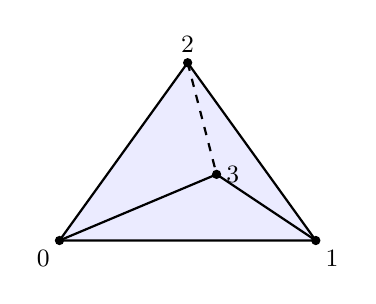
\begin{tikzpicture}[scale=1.05, every node/.style={font=\small}]
        \coordinate (v0) at (-1.55,-0.9);
        \coordinate (v1) at (1.55,-0.9);
        \coordinate (v2) at (0,1.25);
        \coordinate (v3) at (0.35,-0.1);

        \draw[fill=blue!8, draw=none] (v0) -- (v1) -- (v2) -- cycle;
        \draw[thick] (v0) -- (v1) -- (v2) -- cycle;
        \draw[thick] (v0) -- (v3);
        \draw[thick] (v1) -- (v3);
        \draw[thick,dashed] (v2) -- (v3);

        \fill (v0) circle (1.6pt) node[below left] {$0$};
        \fill (v1) circle (1.6pt) node[below right] {$1$};
        \fill (v2) circle (1.6pt) node[above] {$2$};
        \fill (v3) circle (1.6pt) node[right] {$3$};
    \end{tikzpicture}
    \end{center}
    Closing downward adds their edges and vertices. The geometric realization of this complex is homeomorphic to the surface of a sphere, or $S^2$. In that respect it is a \textit{triangulation} of $S^2$. 
\end{example}

Not all topological spaces are triangulable (i.e. have a simplicial complex to which they are homeomorphic), but many interesting ones are. Since we are only working with simplicial complexes we are only able to compute homology for spaces with triangulations, but there are more general notions of homology which apply to all topological spaces.  

\subsection{Homology}

Computing is one way of associating abelian groups to a simplicial complex in a way that gives us important information about their structure. The basic idea is to stop thinking about \textit{geometry} and instead think about formal sums of simplices and record how they meet along their faces. 

Let $K$ be a finite simplicial complex. For each $k\geq 0$, let $K_k$ denote the set of $k$-simplices of $K$. A \textbf{$k$-chain} is a formal integer linear combination of $k$-simplices. The set of all $k$-chains forms the free abelian group $C_k(K) \cong \mathbb Z^{K_k}$.

The next ingredient is the boundary operation. The \textbf{boundary} of a simplex is a formal sum of its codimension-one faces, with signs chosen so that repeated faces cancel when taking the boundary twice. If the vertices of an oriented simplex are ordered as $[v_0,v_1,\dots, v_k]$, then $$\partial_k[v_0,\dots,v_k] = \sum_{i=0}^k (-1)^i[v_0,\dots,\widehat{v_i},\dots, v_k]$$ where the hat means the vertex is omitted. For example, the boundary of an oriented edge $[a,b]$ is $[b]-[a]$ and the boundary of an oriented triangle $[a,b,c]$ is $[b,c]-[a,c] + [a,b]$. Extend this process linearly and we get a group homomorphism $$\partial_k : C_k(K) \to C_{k-1}(K)$$ called the \textbf{boundary map}. 

There are two special kinds of chains. A \textbf{$k$-cycle} is a $k$-chain whose boundary is equal to $0$. A \textbf{$k$-boundary} is a $k$-chain that is the boundary of some $(k+1)$-chain. It happens that for each $k$, $\partial_k\circ\partial_{k+1}=0$, which means that every boundary is a cycle. Algebraically, we have $\text{im }\partial_{k+1} \subseteq \text{ker }\partial_k$. Then we can define the \textbf{$k$th simplicial homology group} of $K$ as the quotient $$H_k(K;\mathbb Z) = \ker \partial_k / \operatorname{im}\partial_{k+1}.$$
 In a few words, homology keeps track of the cycles but thinks of two cycles as equivalent if they differ by a boundary. 

We can think of this as a matrix computation by choosing a basis for each chain group. A natural choice is the set of $k$-simplices, but we need to choose an ordering on this basis as well in order to keep the sign convention consistent. In ChainCert we assume the vertex type comes with a linear order, and takes the lexicographic order on $k$-simplices. With these bases fixed, we can think of each boundary map $\partial_k$ as a matrix of integers. 

\subsection{Using SNF to Compute Simplicial Homology}

Once bases for the chain groups are fixed, each boundary map is represented by
an integer matrix. Suppose that
\[
    \partial_k : \mathbb{Z}^{n_k} \to \mathbb{Z}^{n_{k-1}}
    \qquad\text{and}\qquad
    \partial_{k+1} : \mathbb{Z}^{n_{k+1}} \to \mathbb{Z}^{n_k}
\]
are the two consecutive boundary maps needed to compute $H_k$. The chain
condition says that
\[
    \partial_k \partial_{k+1} = 0,
\]
so every column of the matrix for $\partial_{k+1}$ lies in the kernel of
$\partial_k$.

The first step is to compute the Smith normal form of $\partial_k$. This puts
$\partial_k$ into diagonal form after changing bases in the domain and codomain.
If the diagonal has $r_k$ nonzero entries, then the kernel of $\partial_k$ is a
free abelian group of rank $n_k-r_k$. In the new domain basis, the last
$n_k-r_k$ basis vectors span the cycle group $\ker\partial_k$.

We must then understand the image of $\partial_{k+1}$ as a subgroup of this
cycle group. After applying the same change of basis to the columns of
$\partial_{k+1}$, the first $r_k$ coordinates vanish because
$\partial_k\partial_{k+1}=0$. The remaining $n_k-r_k$ rows form a matrix
\[
    M_k : \mathbb{Z}^{n_{k+1}} \to \mathbb{Z}^{n_k-r_k}
\]
whose image is exactly the boundary subgroup inside the cycle coordinates.
Therefore
\[
    H_k(K;\mathbb{Z})
      \cong \mathbb{Z}^{n_k-r_k} / \operatorname{im} M_k.
\]

Now \Cref{prop:snf-bridge} applies directly to the presentation matrix $M_k$.
If the Smith normal form of $M_k$ has nonzero diagonal entries
$d_1,\ldots,d_s$, then
\[
    H_k(K;\mathbb{Z})
      \cong \mathbb{Z}^{\,n_k-r_k-s}
          \oplus \bigoplus_{i : d_i \text{ is a non-unit}} \mathbb{Z}/d_i\mathbb{Z}.
\]
Over the integers, the non-unit diagonal entries are exactly the torsion
coefficients greater than $1$ up to sign, and the free rank
$n_k-r_k-s$ is the $k$-th Betti number.

This is the computation ChainCert certifies. Sage is used to find the Smith
normal forms, but Lean checks the resulting certificates, checks the chain
condition, constructs the presentation matrix $M_k$, and verifies that the final
read-off of the free rank and torsion coefficients follows from the certified
SNF data.

\section{Certificates}\label{sec:certificates}
\subsection{SNF Certificates}

The basic certificate in ChainCert is an SNF certificate for a matrix. Suppose
$A$ is an $m\times n$ matrix over a PID. Instead of asking Lean to compute the
Smith normal form of $A$, Sage returns the diagonal matrix $D$ together with
change-of-basis matrices $U$ and $V$ and their inverses. Lean then checks that
these matrices really witness a Smith normal form.

\begin{lstlisting}[caption={The core SNF certificate, slightly simplified for display.},label={lst:snf-certificate}]
structure CertificateSNF (A : Matrix (Fin m) (Fin n) R) where
  U    : Matrix (Fin m) (Fin m) R
  Uinv : Matrix (Fin m) (Fin m) R
  V    : Matrix (Fin n) (Fin n) R
  Vinv : Matrix (Fin n) (Fin n) R
  D    : Matrix (Fin m) (Fin n) R
  r    : Nat := firstZeroDiag D

  hrankCutoff : r = firstZeroDiag D
  hdiag  : IsDiagonal D
  hrank  : ∀ i, diagEntry D i = 0 ↔ r <= i.val
  hUUinv : U * Uinv = 1
  hVVinv : V * Vinv = 1
  heq    : U * A * V = D
  hdiv   : ∀ i j, i.val + 1 = j.val →
             diagEntry D i ∣ diagEntry D j
\end{lstlisting}

The fields \lean{U}, \lean{V}, and \lean{D} are the mathematical data of the
Smith normal form: \lean{heq} checks that $D=UAV$. The fields \lean{Uinv} and
\lean{Vinv} make unimodularity checkable by matrix multiplication rather than by
recomputing determinants. The predicate \lean{hdiag} says that $D$ is diagonal,
\lean{hdiv} checks the divisibility chain on consecutive diagonal entries, and
\lean{hrankCutoff} fixes \lean{r} to be the first zero diagonal index.
The field \lean{hrank} records the corresponding zero-tail condition on the
diagonal entries. The number \lean{r} is therefore the rank read off from the
certified diagonal matrix.

All of these fields are small, concrete equations or decidable predicates about
finite matrices. This is the point of the certificate: Sage may have used any
algorithm it likes to find the data, but Lean only needs to check the resulting
matrix identities.

In the current implementation, many of these checks are discharged with
\lean{native_decide}. This is convenient because the goals are finite
computations, but it is not quite the same trust story as a proof by kernel
reduction alone: \lean{native_decide} relies on Lean's native-code evaluator,
and so in principle trusts more of Lean's compiler and runtime. The intended
claim is therefore not that the implementation has Mathlib's smallest possible
trusted base, but that Sage is not trusted for correctness of the mathematical
result. Sage supplies candidate data; Lean checks the certificate data it
receives.

\subsection{Homology Certificates}

The homology certificate packages together the SNF data needed for one degree of
homology. It is stated for two consecutive boundary matrices
\[
    d_k : \mathbb{Z}^{n} \to \mathbb{Z}^{m},
    \qquad
    d_{k+1} : \mathbb{Z}^{p} \to \mathbb{Z}^{n}.
\]
First, it stores an SNF certificate for $d_k$. This identifies coordinates on
the cycle group $\ker d_k$. Second, it checks the chain condition
$d_kd_{k+1}=0$. Third, it stores the presentation matrix $M$ for the image of
$d_{k+1}$ inside those cycle coordinates, together with a proof that this is the
matrix constructed from the certified SNF of $d_k$. Finally, it stores an SNF
certificate for $M$.

\begin{lstlisting}[caption={The chain quotient certificate used to present homology.},label={lst:chain-quotient-certificate}]
structure ChainQuotientCert
    (dk  : Matrix (Fin m) (Fin n) R)
    (dk1 : Matrix (Fin n) (Fin p) R) where
  certK : CertificateSNF dk
  hCC   : dk * dk1 = 0
  M     : Matrix (Fin (n - certK.r)) (Fin p) R
  hM    : M = cyclePresentationMatrix certK dk1
  certM : CertificateSNF M

structure CertificateHomology (X : FFC V) (k : Nat) where
  quotientCert :
    ChainQuotientCert (boundaryK X k) (boundaryK X (k + 1))
\end{lstlisting}

The certificate \lean{ChainQuotientCert} is independent of simplicial complexes:
it is just a certificate for the quotient $\ker d_k/\operatorname{im}d_{k+1}$
associated to two composable matrices. The wrapper \lean{CertificateHomology}
specializes this to the boundary matrices of a finite facet complex. This
separation is useful because the algebraic verification of the quotient does not
depend on how the boundary matrices were produced.

\section{Tactics and Commands}\label{sec:tactics}

ChainCert exposes the Sage bridge through two kinds of interface. Commands such
as \lean{#snf} and \lean{#homology} are exploratory: they ask Sage for a result
and print it in the Lean infoview. Tactics such as \lean{snf} and
\lean{homology} are proof-producing: they call Sage for candidate data, rebuild
that data as Lean expressions, and construct certificates that Lean checks.

\subsection{The \texttt{snf} Tactic}

The \lean{snf} tactic computes a Smith normal form certificate for a concrete
matrix. The basic syntax is:

\begin{lstlisting}[caption={Using the \texttt{snf} tactic.},label={lst:snf-tactic}]
example : True := by
  snf A
  -- cert : CertificateSNF A
  trivial

example : True := by
  snf A as hA
  -- hA : CertificateSNF A
  trivial
\end{lstlisting}

The tactic is goal-agnostic: it adds a certificate to the local context and
leaves the current goal unchanged. Internally, it serializes the entries of
\lean{A}, sends the matrix to Sage, receives matrices \lean{U}, \lean{Uinv},
\lean{D}, \lean{V}, and \lean{Vinv}, and reconstructs a term of type
\lean{CertificateSNF A}. Lean then checks the fields of the certificate by
finite matrix computation, in the current implementation usually through
\lean{native_decide}.

The matrix must have type \lean{Matrix (Fin m) (Fin n) R}, and its entries must
be serializable to Sage. The tactic is intended for concrete matrices whose
entries can be evaluated during elaboration; fully symbolic matrices are not
sent to Sage.

Serialization is handled by the typeclass \lean{SageSerializable}. An instance
specifies how to print elements of a Lean type as Sage-readable strings, how to
parse Sage's string output back into Lean, and the name of the corresponding
Sage ring. The project currently provides instances for \(\mathbb{Z}\) and
\(\mathbb{Q}\). This is an implementation constraint, not a mathematical one:
even if a coefficient ring is a PID in Lean, these Sage-backed tactics can use
it only after a \lean{SageSerializable} instance explains how to translate its
elements to and from Sage. For example:

\begin{lstlisting}[caption={The serialization interface for coefficient rings.},label={lst:sage-serializable}]
class SageSerializable (R : Type*) where
  toSageString   : R -> String
  fromSageString : String -> Option R
  sageName       : String
\end{lstlisting}

This typeclass is deliberately small. Sage's output is not trusted merely
because it parses successfully; parsing only reconstructs candidate matrices.
The certificate fields are still checked in Lean afterward.

\subsection{The \texttt{homology} Tactic}

The \lean{homology} tactic computes a certified homology presentation for a
finite facet complex in one degree. In the examples below,
\lean{triangleFFC} is the finite facet complex on vertices \lean{Fin 3} with a
single facet \(\{0,1,2\}\). In other words, it is the filled triangle
2-simplex, not just its boundary cycle. The syntax mirrors the \lean{snf}
tactic:

\begin{lstlisting}[caption={Using the \texttt{homology} tactic.},label={lst:homology-tactic}]
example : True := by
  homology triangleFFC, 1
  -- homologyCert : CertificateHomology triangleFFC 1
  trivial

example : True := by
  homology triangleFFC, 1 as hTri
  -- hTri : CertificateHomology triangleFFC 1
  trivial

example : CertificateHomology triangleFFC 1 := by
  homology triangleFFC, 1
\end{lstlisting}

When the current goal is already the matching \lean{CertificateHomology} type,
the tactic closes the goal. Otherwise it adds a certificate to the context. The
certificate contains the SNF certificate for the boundary matrix
\(\partial_k\), the checked chain condition
\(\partial_k\partial_{k+1}=0\), the cycle-presentation matrix, and an SNF
certificate for that presentation matrix.

\subsection{Exploratory Commands}

The commands are useful for inspecting Sage output while developing examples.
The command \lean{#snf A} prints the raw SNF data returned by Sage, and
\lean{#homology X, k} prints the homology group Sage computes for the finite
facet complex \lean{X} in degree \lean{k}. These commands are intentionally not
the trusted interface: the trusted path is through the tactics, which turn the
Sage output into Lean-checked certificates.

\section{Theorems}\label{sec:theorems}

The certificate structures are not just records of Sage output. They are meant
to imply the algebraic object we wanted Sage to compute. The formalized theorem
layer is the bridge from executable certificates to ordinary Mathlib algebra:
the certificates contain the low-level matrix equalities, and the theorems
explain what those equalities mean as statements about submodules, cokernels,
and homology quotients.

For SNF certificates, ChainCert proves that the certified row operation is a
linear equivalence and that it identifies the image of the original matrix with
the image of the certified diagonal matrix:

\begin{lstlisting}[caption={A representative bridge theorem for SNF certificates.},label={lst:snf-bridge-theorem}]
theorem map_matRange_eq_diagonal (cert : CertificateSNF A) :
    (matRange A).map
        (rowLinearEquiv (A := A) cert : (Fin m → R) →ₗ[R] (Fin m → R)) =
      matRange cert.D
\end{lstlisting}

As a consequence, an SNF certificate gives exactly the usual object one wants
from Smith normal form: it identifies the cokernel of the original matrix map
with the cokernel of the certified diagonal form. This is the main theorem
connecting the executable SNF certificate to a standard Mathlib quotient
object:

\begin{lstlisting}[caption={The certified diagonal form presents the same cokernel.},label={lst:cokernel-equivalence}]
noncomputable def cokernelEquivDiagonal (cert : CertificateSNF A) :
    ((Fin m → R) ⧸ matRange A) ≃ₗ[R]
      ((Fin m → R) ⧸ matRange cert.D)
\end{lstlisting}

For homology certificates, ChainCert first proves the basic algebraic
consequence of the chain condition: the next boundary image lies in the current
cycle group. This is what makes the quotient
\[
    \ker d_k / \operatorname{im} d_{k+1}
\]
well-defined. ChainCert packages this quotient as a Mathlib object
\lean{homologyModule}. It also proves that the stored presentation matrix has
its own certified diagonal cokernel presentation:

\begin{lstlisting}[caption={The certified homology presentation diagonalizes.},label={lst:homology-presentation-diagonal}]
noncomputable def presentationCokernelEquivDiagonal
    (cert : CertificateHomology X k) :
    ((Fin (cellCount X k - cert.quotientCert.certK.r) → R) ⧸
        matRange cert.presentationMatrix) ≃ₗ[R]
      ((Fin (cellCount X k - cert.quotientCert.certK.r) → R) ⧸
        matRange cert.presentationCert.D)
\end{lstlisting}

Thus, the current certificates already get the central computable object:
a Lean-checked presentation matrix for the homology calculation, together with
a Lean-checked SNF certificate for that presentation. What remains to be
formalized is the clean Mathlib-facing equivalence saying that this presentation
cokernel is the same quotient as \lean{homologyModule}.

The theorem that should eventually be proved is that the presentation matrix
stored in a \lean{ChainQuotientCert} really presents the homology quotient
\(\ker d_k/\operatorname{im}d_{k+1}\). Informally, this should say that the SNF
certificate for \(d_k\) identifies \(\ker d_k\) with the bottom coordinates
after the rank cutoff, and that under this identification the image of
\(d_{k+1}\) is exactly the submodule generated by the columns of the stored
matrix \(M\). Once this equivalence is proved, the existing SNF cokernel theorem
can be composed with it to obtain a fully formal classification of the
certified homology group.

\section{Examples}\label{sec:examples}

\section{Future Work}\label{sec:future}

There are two natural directions for future work.

First, the certificate checks should be moved away from \lean{native_decide}.
The current implementation uses \lean{native_decide} because the relevant goals
are finite matrix computations and native evaluation is fast. However, this
means the trusted base includes Lean's native-code evaluator. A cleaner version
would use verified Boolean checkers, together with reflection theorems of the
form ``the checker returns \lean{true} if and only if the mathematical
predicate holds.'' Some of this infrastructure already exists for diagonal and
boundary verification. There is also now a small constructor,
\lean{CertificateSNF.ofVerifySNF}, which builds a \lean{CertificateSNF} from the
verified SNF predicate. The remaining work is to route the tactic-generated
data through this verified-checker path systematically.

Second, the algebraic theorem layer should be completed. The key missing result
is the equivalence between the actual homology quotient
\(\ker d_k/\operatorname{im}d_{k+1}\) and the cokernel of the certified
cycle-presentation matrix. This is conceptually straightforward linear algebra,
but it requires careful bookkeeping around finite bases, the rank cutoff, and
the coordinate change coming from the SNF certificate for \(d_k\).

The most plausible next theorem is not the full homology classification
theorem, but a lemma isolating the cycle-coordinate statement: after applying
the certified inverse column change for \(d_k\), vectors in \(\ker d_k\) are
exactly those whose first \(r\) coordinates vanish. That lemma would be a
useful stepping stone toward the full presentation theorem.

\section*{Acknowledgments}
The Lean-side Sage transport layer (the persistent subprocess wrapper in \texttt{SageServer.lean}) is adapted from earlier Lean--Sage tactic infrastructure by M.~Karatarakis. The original source is attributed in the file header in the project source.

%\section{Mathematical Background}

%\begin{definition}[Example definition]\label{def:example}
%Let $X$ be a set\ldots
%\end{definition}

%\begin{theorem}[Main result]\label{thm:main}
%For every $n \in \mathbb{N}$, the following holds: $\sum_{k=1}^{n} k = \frac{n(n+1)}{2}$.
%\end{theorem}

%\begin{proof}
%By induction on $n$. The base case is immediate. For the inductive step\ldots
%\end{proof}

%\section{Formalization in Lean}

%The Lean statement corresponding to \Cref{thm:main} is shown below.

%\begin{lstlisting}[caption={Statement of the main theorem.},label={lst:main}]
%theorem sum_range_succ (n : ℕ) :
%    ∑ k in Finset.range (n + 1), k = n * (n + 1) / 2 := by
%  induction n with
%  | zero => simp
%  | succ n ih =>
%    rw [Finset.sum_range_succ, ih]
%    ring
%\end{lstlisting}

%Inline references like \lean{Finset.range} work too.

\bibliographystyle{plain} \bibliography{refs}

\end{document}
